\documentclass [11pt]{article}

\usepackage{amsmath}
\usepackage{amsfonts}
\usepackage{amssymb}
\usepackage{graphicx}
\usepackage{subcaption}
\usepackage{float}
\usepackage{fancyvrb}


\title{INF4490 Mandatory Assignment 1: \\ Travelling Salesman Problem}
\author{Minh Chien Nguyen (davidngcz@gmail.com)}

\begin{document}
\maketitle
\nocite{*}

\section{Introduction}
dfgagf\\
\\
faf
\section{Results}

\subsection{Franke}
\begin{figure}[H]
\centering
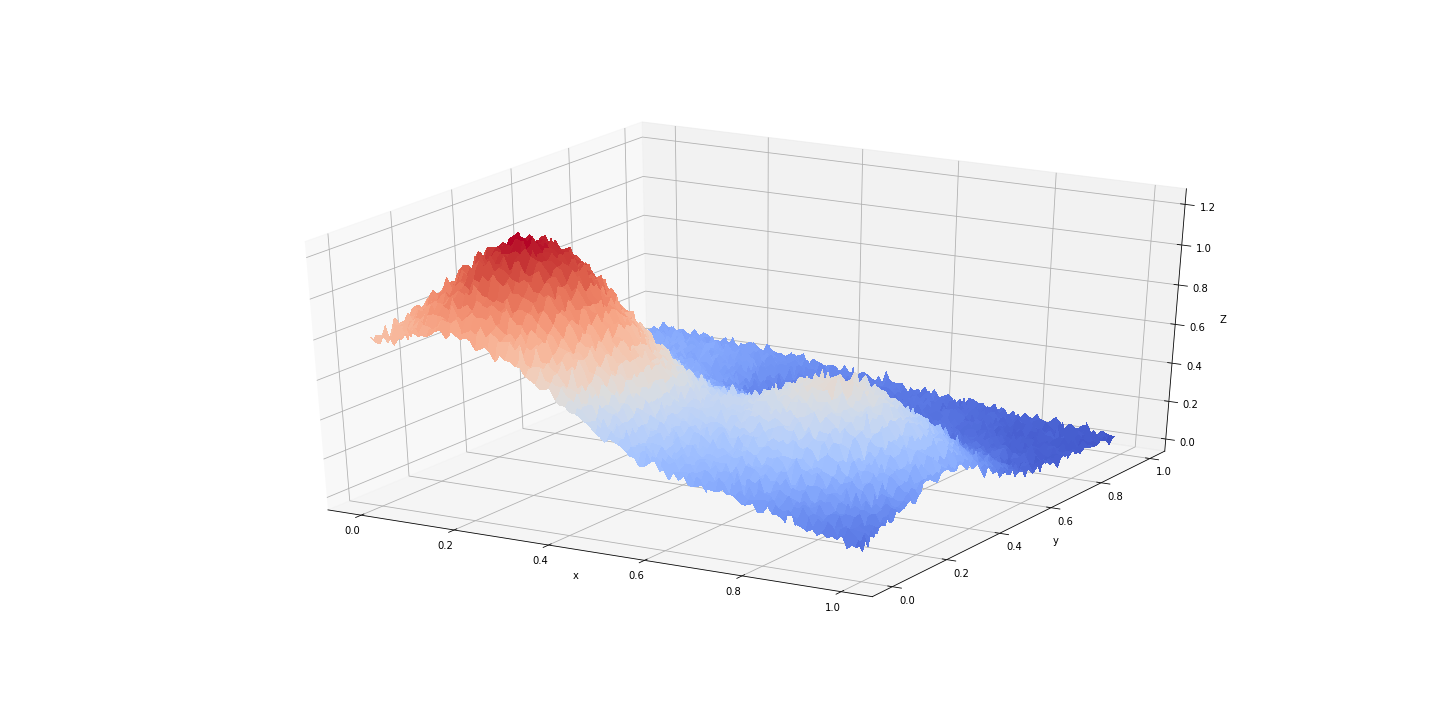
\includegraphics[width=1\textwidth]{figures/Franke.png}
        \caption{Average fitness of the best fit individual in each generation for $24$ cities using Baldwinian GA}
        \label{fig:Franke}
\end{figure}

\subsubsection{OLS}
Table \ref{tab:olsFranke} shows the results obtained using classical OLS method. We see that as the order of the polynomial fit increases the value of  the mean squared error (MSE) decreases, this means that using higher order polynomials is much more accurate. 

\begin{table}[H]
\centering
%\resizebox{\textwidth}{!}{%
\begin{tabular}{lll}
\hline
  & MSE    & R2 score \\ \hline
3 & 0.0082 & 0.9      \\
4 & 0.0044 & 0.94     \\
5 & 0.0025 & 0.97     \\ \hline
\end{tabular}%
%}
\caption{My caption}
\label{tab:olsFranke}
\end{table}
Similarly, there is an increase in the value R-square as the order of polynomial increases. In the case of polynomial fit order $5$, $R^{2}$ is $0.97$, meaning, $97\%$ of variance in $z$ is explained by the predictors. 
\begin{figure}[H]
\centering
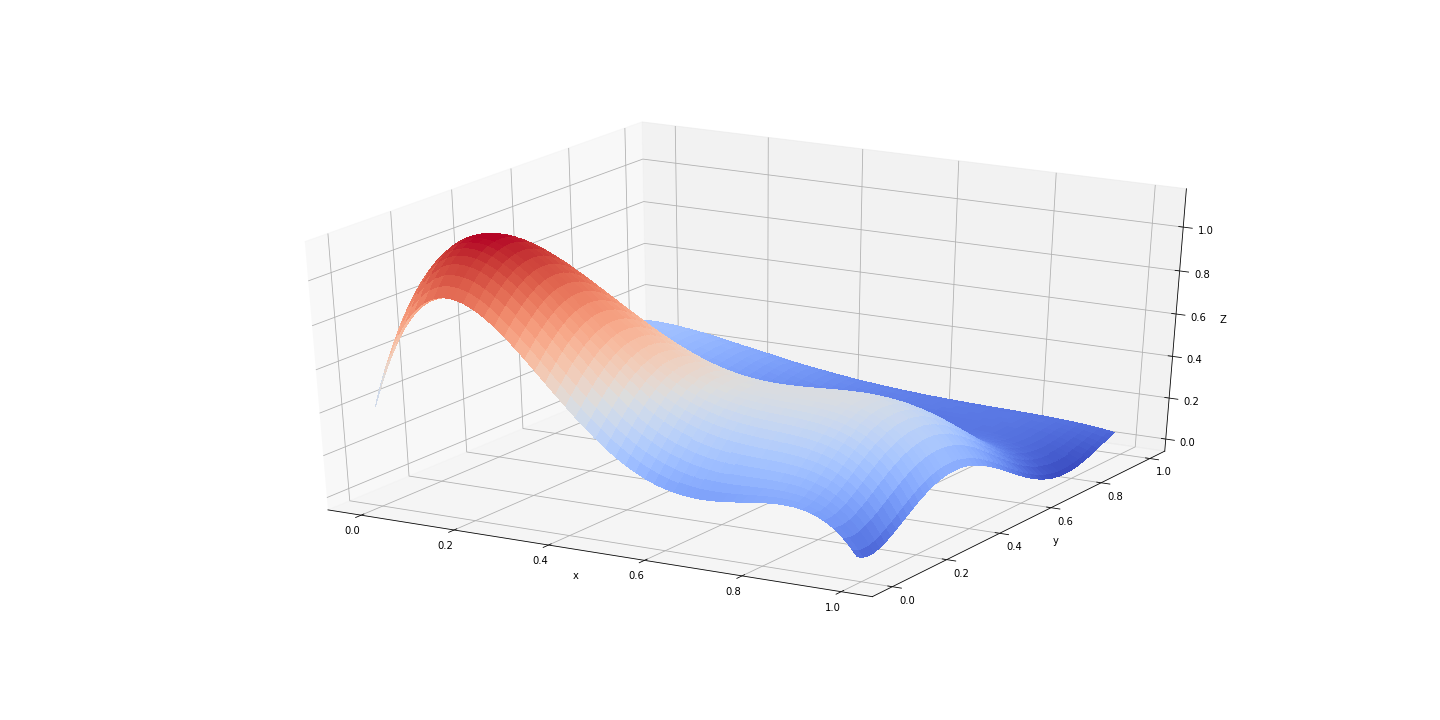
\includegraphics[width=1\textwidth]{figures/olsFranke.png}
        \caption{Average fitness of the best fit individual in each generation for $24$ cities using Baldwinian GA}
        \label{fig:olsFranke}
\end{figure}
Whenever we discuss model prediction, it is important to understand prediction errors (bias and variance). Bias for the final model is: $4.95$ and Variance is: $6.71e-07$. We conclude that our model is underfit neither overfit, since the error of our model is relatively low.


\subsubsection{Ridge}
As mentioned above our model is not overfit, therefore it is not surprising that the best result is obtained using low value of the tuning parameter $\lambda$. In Tables \ref{tab:ridge3}, \ref{tab:ridge4} and \ref{tab:ridge5} we see that as the value of $\lambda$ decreases the value of MSE decreases, meanwhile the coefficient of determination $R^{2}$ is increasing.
\begin{table}[H]
\centering
\begin{tabular}{lll}
\hline
$\lambda$ & MSE    & $R^{2}$ score \\ \hline
0.001     & 0.0082 & 0.90          \\
0.01      & 0.0082 & 0.90          \\
0.1       & 0.0082 & 0.90          \\
1         & 0.0102 & 0.87          \\
10        & 0.0161 & 0.80          \\
100       & 0.0235 & 0.71          \\ \hline
\end{tabular}
\caption{order3}
\label{tab:ridge3}
\end{table}

\begin{table}[H]
\centering
\begin{tabular}{lll}
\hline
$\lambda$ & MSE    & $R^{2}$ score \\ \hline
0.001     & 0.0043 & 0.94          \\
0.01      & 0.0047 & 0.94          \\
0.1       & 0.0071 & 0.91          \\
1         & 0.0091 & 0.88          \\
10        & 0.0137 & 0.83          \\
100       & 0.0223 & 0.73          \\ \hline
\end{tabular}
\caption{order 4}
\label{tab:ridge4}
\end{table}

\begin{table}[H]
\centering
\begin{tabular}{lll}
\hline
$\lambda$ & MSE    & $R^{2}$ score \\ \hline
0.001     & 0.0027 & 0.96          \\
0.01      & 0.0037 & 0.95          \\
0.1       & 0.0056 & 0.93          \\
1         & 0.0089 & 0.89          \\
10        & 0.0124 & 0.85          \\
100       & 0.0213 & 0.74          \\ \hline
\end{tabular}
\caption{order 5}
\label{tab:ridge5}
\end{table}

\begin{figure}[H]
\centering
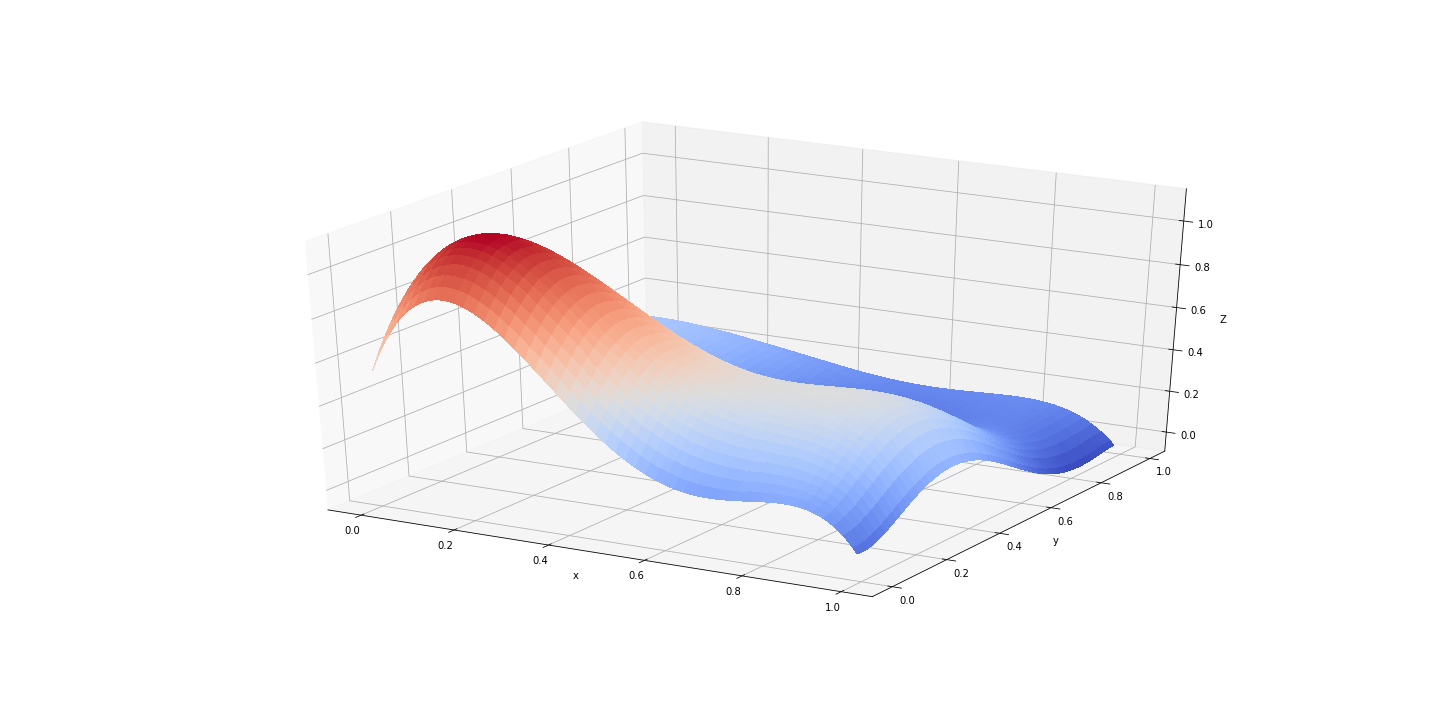
\includegraphics[width=1\textwidth]{figures/RidgeFranke.png}
        \caption{Average fitness of the best fit individual in each generation for $24$ cities using Baldwinian GA}
        \label{fig:RidgeFranke}
\end{figure}
Again, in this case the obtained results of the model using polynomial order $5$ is similar to the results using ordinary OLS model. Bias for the final Rigde model is: $5.18$ and Variance: $4.79e-07$


\subsubsection{Lasso}
Tables \ref{tab:LassoFranke3}, \ref{tab:LassoFranke4} and \ref{tab:LassoFranke5} illustrate the results for Ridge regression using different values of $\alpha$ and orders of polynomials. It is worth mentioning that for some values of $\alpha$ the coefficient of determination $R^{2}$ is negative. The reason is that by increasing $\lambda$ we reduce the magnitude of the coefficients. The higher the values of alpha is , the bigger is the penalty and therefore the magnitude of coefficients are reduced more. However, we also know that our OLS model is not overfit, which means that all predictors in our model are important and by reducing the magnitude of their coefficients we get worse predictions. 


\begin{table}[H]
\centering
\begin{tabular}{lll}
\hline
$\lambda$ & MSE    & $R^{2}$ score \\ \hline
0.001     & 0.0180 & 0.78          \\
0.01      & 0.0254 & 0.69          \\
0.1       & 0.0830 & -0.0011       \\
1         & 0.0830 & -0.0011       \\
10        & 0.0830 & -0.0011       \\
100       & 0.0830 & -0.0011       \\ \hline
\end{tabular}
\caption{3}
\label{tab:LassoFranke3}
\end{table}

\begin{table}[]
\centering
\begin{tabular}{lll}
\hline
$\lambda$ & MSE    & $R^{2}$ score \\ \hline
0.001     & 0.0142 & 0.82          \\
0.01      & 0.0254 & 0.69          \\
0.1       & 0.0830 & -0.0011       \\
1         & 0.0830 & -0.0011       \\
10        & 0.0830 & -0.0011       \\
100       & 0.0830 & -0.0011       \\ \hline
\end{tabular}
\caption{4}
\label{tab:LassoFranke4}
\end{table}

\begin{table}[]
\centering
\begin{tabular}{lll}
\hline
$\lambda$ & MSE    & $R^{2}$ score \\ \hline
0.001     & 0.0135 & 0.83          \\
0.01      & 0.0254 & 0.69          \\
0.1       & 0.0830 & -0.0011       \\
1         & 0.0830 & -0.0011       \\
10        & 0.0830 & -0.0011       \\
100       & 0.0830 & -0.0011       \\ \hline
\end{tabular}
\caption{5}
\label{tab:LassoFranke5}
\end{table}

\begin{figure}[H]
\centering
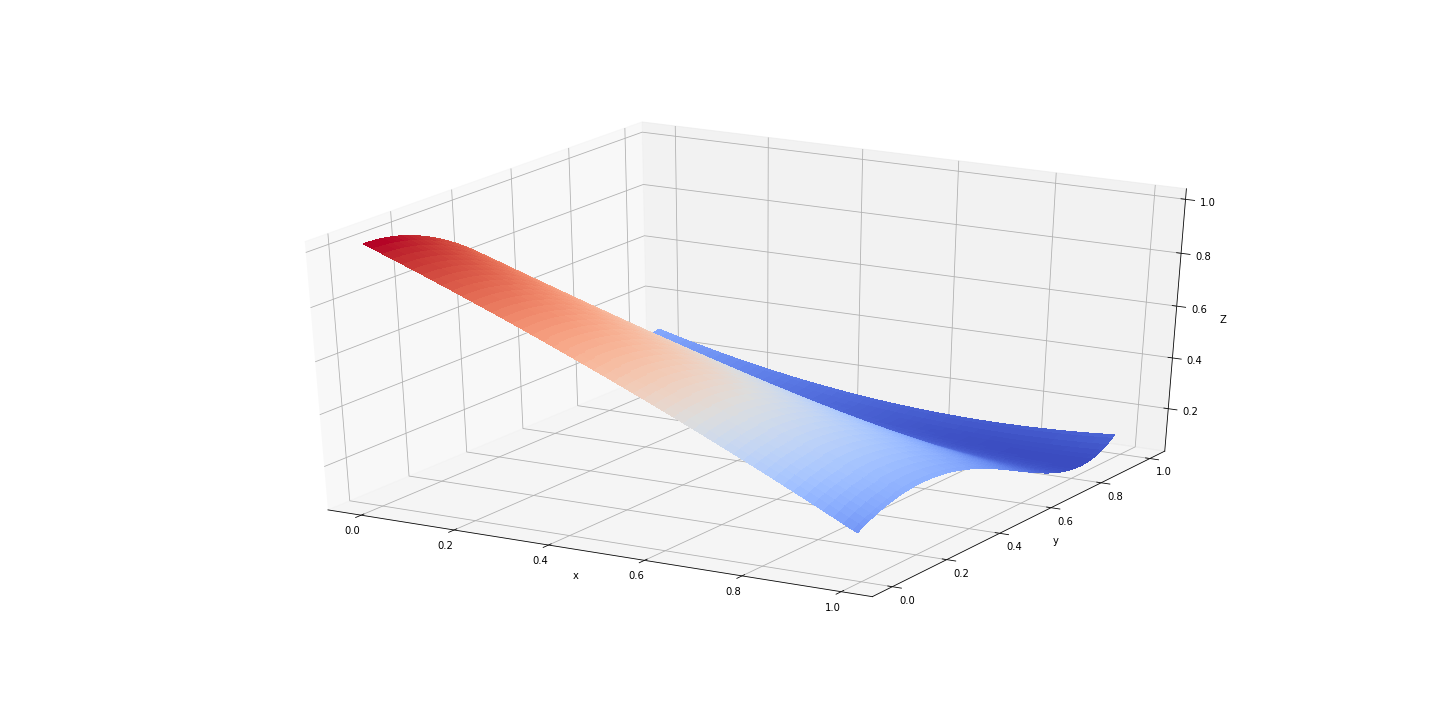
\includegraphics[width=1\textwidth]{figures/LassoFranke.png}
        \caption{Average fitness of the best fit individual in each generation for $24$ cities using Baldwinian GA}
        \label{fig:LassoFranke}
\end{figure}

Bias for the best Lasso model is $13.56$ and Variance is $1.04e-06$. We can see that, both values for the Lasso model has been increased in comparison with the OLS and Ridge model. Therefore, in this case Lasso model is predicting worse than both OLS and Ridge.

\begin{thebibliography}{111}
\raggedright
\bibitem{abc} EIBEN, Agoston E., et al. Introduction to evolutionary computing. Berlin: springer, 2003.
\bibitem{def} MARSLAND, Stephen. Machine learning: an algorithmic perspective. Chapman and Hall/CRC, 2011.

\end{thebibliography}
\end{document}